\medskip

\textbf{PARTIE A}

\medskip

\begin{enumerate}
\item
	\begin{enumerate}
		\item Pour tout réel $x$ de l'intervalle $[0~;~\pi]$ :

$f'(x) = \e^x \times \sin(x) +\e^x \times  \cos(x) = \e^x \big( \sin(x) +\cos(x)\big)$.
		\item Par connaissance des fonctions trigonométriques, pour tout réel $x$ de l'intervalle $\left[0~;~\dfrac{\pi}{2}\right]$,\quad $\cos(x)\geqslant 0$ et $\sin(x)\geqslant 0$

On précise que d'une part, $\sin(x) = 0$ seulement pour $x = 0$, et $cos(0) = 1$, et d'autre part, $\cos(x) = 0$ seulement pour $x = \dfrac{\pi}{2}$, et $\sin\left(\dfrac{\pi}{2}\right)  =1$, donc les fonctions sinus et cosinus ne s'annulent pas en même temps.

La somme de deux réels positifs, dont l'un au moins est strictement positif est strictement positive, donc:

pour tout réel $x$ de l'intervalle $\left[0~;~\dfrac{\pi}{2}\right]$, \quad $\cos(x)+ \sin(x)> 0$.

D'autre part, pour tout réel $x$,\, $\e^{x} > 0$

donc pour tout réel $x$ de l'intervalle $\left[0~;~\dfrac{\pi}{2}\right]$,\quad $f'(x)> 0$ \quad en tant que produit de deux facteurs strictement positifs,

donc  la fonction $f$ est strictement croissante sur l'intervalle  $\left[0~;~\dfrac{\pi}{2}\right]$.
	\end{enumerate}
\item
	\begin{enumerate}
		\item L'équation réduite de la tangente à la courbe $\mathcal{C}_f$ au point d'abscisse 0 est : $y =f'(0)(x - 0) + f(0) = f'(0)x + f(0)$.

$f(0) = \e^0 \sin (0)= 1 \times 0= 0$ ; (donné dans l'énoncé)

$f'(0)= \e^0 \left( \sin(0) +\cos(0)\right) = 1 \times(0+1)=1$ (donné dans l'énoncé)

L'équation de la tangente $T$ à la courbe $\mathcal{C}_f$ au point d'abscisse~$0$ est donc $y = 1x + 0$ soit $y=x$.

		\item En anticipant la question \textbf{3.}, on va étudier la convexité de la fonction sur $[0 ~;~ \pi]$.

Pour tout réel $x$ de l'intervalle $\left[0~;\pi\right]$ :

$\begin{aligned}
f''(x) & = \e^x \left( \sin(x) +\cos(x)\right)  + \e^x\left( \cos(x) -\sin(x)\right)\\
	& = \e^x \left( \sin(x) +\cos(x) +\cos(x) -\sin(x)\right)\\
	&= 2 \e^x \cos(x)
\end{aligned}$.

On a le tableau de signes suivant :

\hfill~\begin{tikzpicture}
			\tkzTabInit[lgt=3,espcl=3]{$x$/0.7,
				signe de $f''(x)$/0.7}{$0$,$\frac{\pi}{2}$,$\pi$}
			\tkzTabLine{,+,z,-,}
		\end{tikzpicture}\hfill~

donc pour tout réel $x$ de l'intervalle $\left[0~;~\dfrac{\pi}{2}\right]$, $f''(x)>0$

d'où la fonction $f$ est convexe sur l'intervalle  $\left[0~;~\dfrac{\pi}{2}\right]$.
		\item La courbe représentative d'une fonction convexe est au-dessus de toutes ses tangentes, en particulier ici, la courbe $\mathcal{C}_f$  est au-dessus de la tangente à la courbe $\mathcal{C}_f$ au point d'abscisse 0, d'équation $y = x$ (d'après la question précédente).

On a donc, pour tout réel $x$ de l'intervalle $\left[0~;~\dfrac{\pi}{2}\right]$,\quad $\e^x \sin (x) \geqslant x$.
	\end{enumerate}
\item On a vu précédemment que la dérivée seconde de $f$ s'annule en changeant de signe en $x=\dfrac{\pi}{2}$ donc le point d'abscisse $\dfrac{\pi}{2}$ de la courbe représentative de la fonction $f$ est un point d'inflexion.
\end{enumerate}

\bigskip

\textbf{PARTIE B}

\medskip


On note

\[I = \displaystyle\int_0^{\frac{\pi}{2}} \e^x \sin (x)\, \text{d}x\quad  \text{et}\quad J = \displaystyle\int_0^{\frac{\pi}{2}} \e^x \cos (x)\, \text{d}x.\]

\smallskip

\begin{enumerate}
\item

$x \longmapsto \e^x \sin(x)$ est de la forme $u v'$ avec $\begin{cases}u(x)=\e^x \quad\text { et }  \quad u'(x)=\e^x \\ v'(x)=\sin(x) \quad\text { et } \quad v(x)=-\cos(x)\end{cases}$

Les fonctions $u$ et $v$ sont continues et dérivables sur $\left[0~;~\dfrac{\pi}{2}\right]$ et les fonctions $u'$ et $v'$ sont continues sur $\left[0~;~\dfrac{\pi}{2}\right]$, donc, d'après la formule d'intégration par parties :

$\displaystyle \int_{a}^{b} u(x)v'(x)\, \mathrm{d}x = \Big [ u(x)v(x)\strut\Big]_{a}^{b} - \int_{a}^{b} u'(x)v(x) \, \mathrm{d}x$.

d'où 
$\begin{aligned}[t]
	I & =\Big[-\cos(x)\e^x\Big]_0^{\frac{\pi}{2}}-\int_0^{\frac{\pi}{2}} \e^x(-\cos(x))  \, \mathrm{d}x\\
	& = -\cos \left(\dfrac{\pi}{2}\right)\e^{\frac{\pi}{2}}+\cos(0)\e^0+\int_0^{\frac{\pi}{2}} \e^x\cos(x) \, \mathrm{d}x\\
	& =0+1+J\\
	& =1+ J
\end{aligned}$

\smallskip

$x \longmapsto \e^x \sin(x)$ est de la forme $u v'$ avec $\begin{cases}u(x)=\sin(x) \quad\text { et }\quad u'(x)=\cos(x)\\ v'(x)=\e^x \quad \text { et } \quad v(x)=\e^x \end{cases}$

Les fonctions $u$ et $v$ sont continues et dérivables sur $\left[0~;~\dfrac{\pi}{2}\right]$ et  les fonctions $u'$ et $v'$ sont continues sur $\left[0~;~\dfrac{\pi}{2}\right]$, donc, d'après la formule d'intégration par parties :
$\displaystyle \int_{a}^{b} u(x)v'(x)\, \mathrm{d}x = \Big [ u(x)v(x)\Big]_{a}^{b} - \int_{a}^{b} u'(x)v(x) \, \mathrm{d}x$.

d'où 
$\begin{aligned}[t]
	I & =\Big[\sin(x)\e^x\Big]_0^{\frac{\pi}{2}}-\int_0^{\frac{\pi}{2}} \e^x\cos(x)  \, \mathrm{d}x \\
	& = -\sin \left(\dfrac{\pi}{2}\right)\e^{\frac{\pi}{2}}+\sin(0)\e^0-J\\
	& =\e^{\frac{\pi}{2}} - J
\end{aligned}
$

On a donc bien :
\[I= 1+J \qquad \text{et}\qquad I= \e^{\frac{\pi}{2}} - J.\]

\item En ajoutant les deux équations précédentes on obtient : $2I = 1 +J + \e^{\frac{\pi}{2}}-J $.

d'où  $I = \dfrac{1 + \e^{\frac{\pi}{2}}}{2}$.

\item D'après la question \textbf{Partie A 2.c.} pour tout réel $x$ de l'intervalle $\left[0~;~\dfrac{\pi}{2}\right]$,

$\e^x \sin (x) \geqslant x$ c'est à dire $f(x) \geqslant g(x)$.

L'aire du domaine hachuré situé entre les courbes $\mathcal{C}_f$ et $\mathcal{C}_g$ et les droites d'équation $x = 0$ et $x = \dfrac{\pi}{2}$ est donc égale à l'intégrale : $\displaystyle   \int_0^{\frac{\pi}{2}} \left( \e^x \sin (x)-x\right)\, \text{d}x$.

$\begin{aligned}
	\displaystyle \mathcal{A} & = \int_0^{\frac{\pi}{2}} \left(\e^x \sin (x)-x\right)\, \text{d}x\\
	&= \displaystyle\int_0^{\frac{\pi}{2}} \e^x \sin (x)\, \text{d}x - \displaystyle\int_0^{\frac{\pi}{2}} x\, \text{d}x \quad  \text{ par linéarité de l'intégrale} \\
	& = I - \left[ \frac{x^2}{2}\right]_0^{\frac{\pi}{2}}\\
	& = \dfrac{1 + \e^{\frac{\pi}{2}}}{2}- \dfrac{1}{2}{\left( \dfrac{\pi}{2} \right)}^2+0\\
	& = \dfrac{1 + \e^{\frac{\pi}{2}}}{2}-  \dfrac{\pi^2}{8}
\end{aligned}$

L'aire cherchée est donc \quad $ \dfrac{1 + \e^{\frac{\pi}{2}}}{2} - \dfrac{\pi^2}{8}$ u.a. ($\approx 1,67$ u. a.)
\end{enumerate}

\begin{center}
\psset{xunit=2.4cm,yunit=1.2cm,arrowsize=2pt 3}
\begin{pspicture}(-1,-1)(4,9)
\multido{\n=0.0+0.5}{6}{\psline[linewidth=0.35pt,linecolor=orange](\n,0)(\n,8)}
\multido{\n=0.0+0.5}{17}{\psline[linewidth=0.35pt,linecolor=orange](0,\n)(3,\n)}
\psaxes[linewidth=1.25pt,Dy=2,labelFontSize=\scriptstyle]{->}(0,0)(0,0)(4,9)
\psline[linestyle=dotted,linewidth=2pt](1.5708,0)(1.5708,1.5708)
\psline[linewidth=1.25pt](1.5708,1.5708)(1.5708,4.81)
\psplot[plotpoints=1500,linewidth=1.25pt,linecolor=blue]{0}{3.14159}{2.71828 x exp x 180 mul 3.14159 div sin mul}
\psplot[plotpoints=1500,linewidth=1.25pt]{0}{3.14159}{x}
\uput[ur](2.7,6.6){\blue $\mathcal{C}_f$}\uput[dr](2.54,2.6){$\mathcal{C}_g$}
\pscustom[fillstyle=vlines]{\psplot[plotpoints=1500,linewidth=1.25pt,linecolor=blue]{0}{1.5708}{2.71828 x exp x 180 mul 3.14159 div sin mul}\psline[linewidth=1.25pt](1.5708,4.81)(1.5708,1.5708)(0,0)}
\end{pspicture}
\end{center}
